% Adjust these for the path of the theme and its graphics, relative to this file
%\usepackage{beamerthemeFalmouthGamesAcademy}
\usepackage{../../beamerthemeFalmouthGamesAcademy}
\usepackage[utf8]{inputenc}
\usepackage{multimedia}
\graphicspath{ {../../} }

% Default language for code listings
\lstset{language=Python,
    keepspaces=true,
    breaklines=false
}

% For strikethrough effect
\usepackage[normalem]{ulem}
\usepackage{wasysym}

\usepackage{algpseudocode}

\usepackage{pdfpages}

\usepackage{circuitikz}

\iftoggle{printable}{
    \newcommand{\circuitcolour}{black}
}{ % else
    \newcommand{\circuitcolour}{white}
}

% http://www.texample.net/tikz/examples/state-machine/
\usetikzlibrary{arrows,automata}

\newcommand{\modulecode}{COMP140 GAM160}\newcommand{\moduletitle}{Hacking Hardware/Advanced Programming}\newcommand{\sessionnumber}{Session 6}

\hypersetup{
pdftex,
pdftitle=\sessionnumber: Data Types,
pdfauthor=Ed Powley,
pdfdisplaydoctitle,
pdflang=en-GB
}
 
\begin{document}
\title{\sessionnumber: Data Types}
\subtitle{\modulecode: \moduletitle}

\frame{\titlepage} 

\part{Binary notation}
\frame{\partpage}

\begin{frame}
	\centering
	\includegraphics[width=0.7\textwidth]{10-types-of-people}
	\par\vspace{2ex}\par
	{\tiny Image credit: \url{http://www.toothpastefordinner.com}}
\end{frame}



\begin{frame}{How we write numbers}
	\begin{itemize}
		\pause\item We write numbers in \textbf{base~10}
		\pause\item We have 10 \textbf{digits}: $0, 1, 2, \dots, 8, 9$
		\pause\item When we write $6397$, we mean:
			\begin{itemize}
				\pause\item Six thousand, three hundred and ninety seven
				\pause\item (Six thousands) and (three hundreds) and (nine tens) and (seven)
				\pause\item $(6 \times 1000) + (3 \times 100) + (9 \times 10) + (7)$
				\pause\item $\left(6 \times 10^3\right)
				+ \left(3 \times 10^2\right)
				+ \left(9 \times 10^1\right)
				+ \left(7 \times 10^0\right)$
				\pause\item
				    \begin{tabular}{cccc}
				        Thousands & Hundreds & Tens & Units \\
				        6 & 3 & 9 & 7
				    \end{tabular}
			\end{itemize}
	\end{itemize}
\end{frame}

\begin{frame}{Binary}
	\begin{itemize}
		\pause\item Binary notation works the same, but is \textbf{base~2} instead of \textbf{base~10}
		\pause\item We have 2 \textbf{digits}: $0, 1$
		\pause\item When we write $10001011$ in binary, we mean: \par\pause
			$\phantom{+} \left(1 \times 2^7\right) + 
			\left(0 \times 2^6\right) + 
			\left(0 \times 2^5\right) + 
			\left(0 \times 2^4\right)$ \par
			$+ \left(1 \times 2^3\right) + 
			\left(0 \times 2^2\right) + 
			\left(1 \times 2^1\right) + 
			\left(1 \times 2^0\right)$ \par\pause
			$= 2^7 + 2^3 + 2^1 + 2^0$ \par\pause
			$= 128 + 8 + 2 + 1 \text{ (base 10)}$ \par\pause
			$= 139 \text{ (base 10)}$
	\end{itemize}
\end{frame}

\begin{frame}{Converting to binary}
    \begin{center}
        \url{https://www.youtube.com/watch?v=OezK_zTyvAQ}
    \end{center}
\end{frame}

\begin{frame}{Bits, bytes and words}
	\begin{itemize}
		\pause\item A \textbf{bit} is a \uline{b}inary dig\uline{it}
			\begin{itemize}
				\pause\item Can store a 0 or 1 (i.e.\ a boolean value)
			\end{itemize}
		\pause\item A \textbf{byte} is 8 \textbf{bits}
			\begin{itemize}
				\pause\item Can store a number between 0 and 255 in binary
			\end{itemize}
		\pause\item A \textbf{word} is the number of bits that the CPU works with at once
			\begin{itemize}
				\pause\item 32-bit CPU: 32 bits = 1 word
				\pause\item 64-bit CPU: 64 bits = 1 word
			\end{itemize}
		\pause\item An $n$-bit word can store a number between 0 and $2^{n} - 1$
			\begin{itemize}
				\pause\item $2^{16}-1 = 65,535$
				\pause\item $2^{32}-1 = 4,294,967,295$
				\pause\item $2^{64}-1 = 18,446,744,073,709,551,615$
			\end{itemize}
	\end{itemize}
\end{frame}

\newcommand{\carry}[1]{\uncover<#1->{$_1$}}
\newcommand{\nocarry}[1]{\phantom{$_1$}}

\begin{frame}{Addition with carry}
	In base 10:
	\begin{center}
		\begin{tabular}{lllll}
			& 1 & 2 & 3 & 4 \\
			+ & 5\nocarry{4} & 6\carry{3} & 7\carry{2} & 8\nocarry{1} \\\hline
			& \uncover<5->{6} & \uncover<4->{9} & \uncover<3->{1} & \uncover<2->{2}
		\end{tabular}
	\end{center}
\end{frame}

\begin{frame}{Addition with carry}
	In base 2:
	\begin{center}
		\fbox{$1 + 1 = 10$ \qquad $1 + 1 + 1 = 11$}
		
		\vspace{2ex}
		
		\begin{tabular}{lllllllll}
			& 0 & 1 & 1 & 0 & 1 & 1 & 1 & 0 \\
			+ &
				0\carry{8} &
				0\carry{7} &
				1\nocarry{6} &
				0\carry{5} &
				0\carry{4} &
				1\carry{3} &
				1\nocarry{2} &
				1 \\\hline
			&
				\uncover<9->{1} &
				\uncover<8->{0} &
				\uncover<7->{0} &
				\uncover<6->{1} &
				\uncover<5->{0} &
				\uncover<4->{1} &
				\uncover<3->{0} &
				\uncover<2->{1}
		\end{tabular}
	\end{center}
\end{frame}

\begin{frame}{Modular arithmetic}
    \begin{columns}
        \begin{column}{0.4\textwidth}
            \begin{center}
                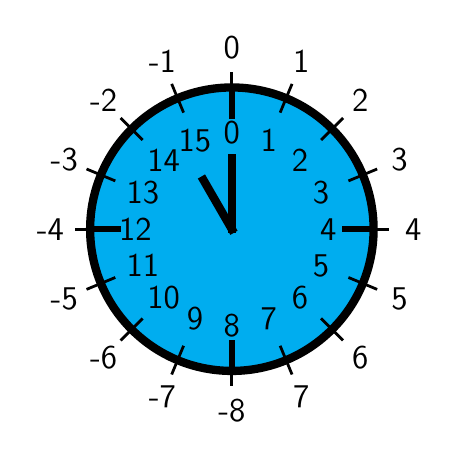
\begin{tikzpicture}[line cap=rect,line width=3pt,scale=0.9]
                    \filldraw [fill=cyan] (0,0) circle [radius=2cm];
                    \foreach \angle [count=\xi from 0] in {90,67.5,...,-247.5}
                    {
                        \draw[line width=1pt] (\angle:1.8cm) -- (\angle:2.2cm);
                        \node[font=\large] at (\angle:1.36cm) {\textsf{\xi}};
                    }
                    \foreach \angle [count=\xi from -8] in {270,247.5,...,-67.5}
                    {
                        \node[font=\large] at (\angle:2.56cm) {\textsf{\xi}};
                    }
                    \foreach \angle in {0,90,180,270}
                        \draw[line width=2pt] (\angle:1.6cm) -- (\angle:2cm);
                    \draw (0,0) -- (120:0.8cm);
                    \draw (0,0) -- (90:1cm);
                \end{tikzpicture}
            \end{center}
        \end{column}
        \begin{column}{0.55\textwidth}
            \begin{itemize}
                \pause\item Arithmetic \textbf{modulo} $N$
                \pause\item Numbers ``wrap around'' between $0$ and $N-1$
                \pause\item E.g.\ modulo $16$:
                    \begin{itemize}
                        \pause\item $14 + 7 = 5$
                        \pause\item $4 - 7 = 13$
                    \end{itemize}
            \end{itemize}
        \end{column}
    \end{columns}
\end{frame}

\begin{frame}{2's complement}
    \begin{itemize}
        \pause\item How can we represent negative numbers in binary?
        \pause\item Represent them modulo $2^n$ (for $n$ bits)
        \pause\item I.e.\ represent $-a$ as $2^n-a$
        \pause\item Instead of an $n$-bit number ranging from $0$ to $2^n-1$, it ranges from $-2^{n-1}$ to $+2^{n-1}-1$
        \pause\item E.g.\ 16-bit number ranges from $-32768$ to $+32767$
        \pause\item Note that the left-most bit can be interpreted as a \textbf{sign} bit:
            $1$ if negative, $0$ if positive or zero
    \end{itemize}
\end{frame}

\begin{frame}{Converting to 2's complement}
    \begin{itemize}
        \pause\item Convert the absolute value to binary
        \pause\item Invert all the bits (i.e.\ change $0 \leftrightarrow 1$)
        \pause\item Add 1
        \pause\item (This is equivalent to subtracting the number from $2^n$... why?)
        \pause\item This is also the process for converting back from 2's complement,
            i.e.\ doing it twice should give the original number
    \end{itemize}
\end{frame}

\begin{frame}{Why 2's complement?}
    \begin{itemize}
        \pause\item Allows all addition and subtraction to be carried out modulo $2^n$
            without caring whether numbers are positive or negative
        \pause\item In fact, subtraction can just be done as addition
        \pause\item I.e.\ $a-b$ is the same as $a+(-b)$, where $a$ and $-b$ are just $n$-bit numbers
    \end{itemize}
\end{frame}

\part{Numeric types}
\frame{\partpage}

\begin{frame}{Integers}
	\begin{itemize}
		\pause\item An \textbf{integer} is a whole number --- positive, negative or zero
		\pause\item Stored in memory using binary notation, with 2's complement for negative values
		\pause\item In C\#: \csinline{int} is a 32-bit integer, \csinline{long} is a 64-bit integer
		\pause\item In Python: \lstinline{int} is a ``big integer'' --- expands number of bits automatically to fit the value to be stored
	\end{itemize}
\end{frame}

\begin{frame}{Floating point numbers}
	\begin{itemize}
		\pause\item What about storing non-integer numbers?
		\pause\item Usually we use \textbf{floating point} numbers
		\pause\item Details on in-memory representation later in the module
		\pause\item In C\#: \csinline{float} or \csinline{double}
		\pause\item \csinline{double} is more precise, but uses twice as much memory (8 bytes vs 4 bytes)
		\pause\item Python type: \lstinline{float}, which has the same precision as C\# \lstinline{double}!
	\end{itemize}
\end{frame}

\begin{frame}{Integers vs floating point numbers}
	\begin{itemize}
		\pause\item Integers and floating point numbers are \textbf{different types}!
		\pause\item \csinline{42} and \csinline{42.0} are technically different values
			\begin{itemize}
				\pause\item One is an \csinline{int}, the other is a \csinline{double}
				\pause\item They are stored differently in memory (completely different sequences of bytes)
				\pause\item However, \csinline{==} etc still know how to compare them sensibly
			\end{itemize}
	\end{itemize}
\end{frame}

% \begin{frame}{Other number formats}
% 	\begin{itemize}
% 		\pause\item \textbf{Fixed point}: alternative format for non-integer numbers
%             \begin{itemize}
%                 \pause\item More on this later
%                 \pause\item E.g.\ \lstinline{decimal} module in Python
%             \end{itemize}
%         \pause\item \textbf{Rational numbers}: store fractions as numerator and denominator
%             \begin{itemize}
%                 \pause\item E.g.\ \lstinline{fractions} module in Python
%             \end{itemize}
%         \pause\item \textbf{Complex numbers}: stored as a pair of floating point numbers for real and imaginary parts
%             \begin{itemize}
%                 \pause\item E.g.\ \lstinline{complex} type in Python
%             \end{itemize}
% 	\end{itemize}
% \end{frame}


\part{String types}
\frame{\partpage}

\begin{frame}{Strings}
	\begin{itemize}
		\pause\item A \textbf{string} represents a sequence of textual characters
		\pause\item E.g.\ \lstinline{"Hello world!"}
		\pause\item Python type: \lstinline{str}
	\end{itemize}
\end{frame}

\begin{frame}{String representation}
	\begin{itemize}
		\pause\item Stored as sequences of \textbf{characters} encoded as \textbf{integers}
		\pause\item Often \textbf{null-terminated}
			\begin{itemize}
				\pause\item Character number 0 signifies the end of the string
			\end{itemize}
	\end{itemize}
\end{frame}

\begin{frame}{What is a character?}
	\begin{itemize}
		\pause\item Broadly speaking, a single \textbf{printable symbol}
		\pause\item There are also some special \textbf{non-printable characters} e.g.\ line break
	\end{itemize}
\end{frame}

\begin{frame}{ASCII}
	\begin{itemize}
		\pause\item American Standard Code for Information Interchange
		\pause\item Defines a standard set of 128 characters (7 bits per character)
		\pause\item Originally developed in the 1960s for teletype machines, but survives in computing to this day
		\pause\item 95 printable characters: upper and lower case English alphabet, digits, punctuation
		\pause\item 33 non-printable characters
	\end{itemize}
\end{frame}

{
\setbeamercolor{background canvas}{bg=white}
\begin{frame}[plain]
	\begin{tikzpicture}[remember picture, overlay]
		\node[at=(current page.center)] {
			\includegraphics[width=\paperwidth]{ascii_chart_2}
		};
	\end{tikzpicture}
\end{frame}
}

\begin{frame}{ASCII}
	\begin{itemize}
		\pause\item ASCII works OK for English
		\pause\item Standards exist to add another 128 characters (taking us to 8 bits per character)
		\pause\item E.g.\ accented characters for European languages, other Western alphabets e.g. Greek, Cyrillic,
		    mathematical symbols
		\pause\item However 256 characters isn't enough...
	\end{itemize}
\end{frame}

\begin{frame}{Unicode}
	\begin{itemize}
		\pause\item Standard character set developed from 1987 to present day
		\pause\item Currently defines 137994 characters (Unicode 12.1)
		\pause\item First 128 characters are the same as ASCII
		\pause\item Covers most of the world's writing systems
		\pause\item Also covers mathematical symbols and emoji
	\end{itemize}
\end{frame}

\begin{frame}{Encoding Unicode}
    \begin{itemize}
		\pause\item \textbf{UTF-32} encodes characters as 32-bit integers
		\pause\item \textbf{UTF-8} encodes characters as 8, 16, 24 or 32-bit integers
			\begin{itemize}
			    \pause\item 8-bit characters correspond to the first 128 ASCII characters
			        $\implies$ backwards compatible
				\pause\item More common Unicode characters are smaller
				    $\implies$ more efficient than UTF-32
			\end{itemize}
	\end{itemize}
\end{frame}

\begin{frame}{String representation}
	\begin{itemize}
		\pause\item \lstinline{"Hello world!"} in ASCII or UTF-8 encoding:
	\end{itemize}
	
	{\footnotesize\pause\begin{tabular}{*{13}{|c}|}
		\hline
		72 & 101 & 108 & 108 & 111 & 32 & 119 & 111 & 114 & 108 & 100 & 33 & 0 \\\hline
	\end{tabular}}
\end{frame}

\begin{frame}{UTF-8 representation}
	\begin{itemize}
		\pause\item For characters in ASCII, UTF-8 is the same:
			\begin{itemize}
				\pause\item a $\to [97]$
			\end{itemize}
		\pause\item Other characters are encoded as multi-byte sequences:
			\begin{itemize}
				\pause\item \"u $\to [195, 188]$
				\pause\item \includegraphics[height=1.5ex]{chinese}\ $\to [228, 184, 178]$
				\pause\item \includegraphics[height=1.5ex]{emoji}\ $\to [240, 159, 152, 130]$
			\end{itemize}
		\pause\item \texttt{"Haha \includegraphics[height=1.5ex]{emoji}"} encoded in UTF-8:
	\end{itemize}
	{\footnotesize\pause\begin{tabular}{*{13}{|c}|}
		\hline
		H & a & h & a & space & \multicolumn{4}{c|}{\includegraphics[height=1.5ex]{emoji}} & null \\\hline
		72 & 97 & 104 & 97 & 32 & 240 & 159 & 152 & 130 & 0 \\\hline
	\end{tabular}}
\end{frame}

\begin{frame}{Strings in Python}
    \begin{itemize}
        \pause\item Python 2 had separate types for ASCII and Unicode strings: \lstinline{str} and \lstinline{unicode}
        \pause\item Python 3 has just the \lstinline{str} type, which uses Unicode
        \pause\item String literals are wrapped in \lstinline{'single quotes'} or \lstinline{"double quotes"}
            (there is no difference)
    \end{itemize}
\end{frame}

\begin{frame}[fragile]{Escape sequences}
    \begin{itemize}
        \pause\item Backslash \textbackslash\ has a special meaning in string literals
            --- it denotes the start of an \textbf{escape sequence}
        \pause\item Typically used to write \textbf{non-printable characters}
        \pause\item Most useful: \lstinline{"\n"} is a new line
        \pause\item How to type a backslash character? Use \lstinline{"\\"}
    \end{itemize}
\end{frame}

\begin{frame}{String literal tricks in Python}
    \begin{itemize}
        \pause\item Use triple quotes \lstinline{'''} or \lstinline{"""} for a multi-line string
        \pause\item Use \lstinline{r" "} or \lstinline{r' '} to turn off escape characters
            (useful for strings with lots of backslashes, e.g.\ Windows file paths, regular expressions)
    \end{itemize}
\end{frame}

\begin{frame}[fragile]{Text files}
    \begin{itemize}
        \pause\item Stored on disk as essentially one long string
        \pause\item Line endings are denoted by non-printable characters
            \begin{itemize}
                \pause\item Unix format: line feed character (ASCII/UTF-8 character 10, \lstinline{"\n"})
                \pause\item Windows format: carriage return character (ASCII/UTF-8 character 13) followed by line feed, \lstinline{"\r\n"}
                \pause\item Most text editors can handle and convert both formats
                \pause\item Most languages allow files to be opened in ``text mode'' which automatically converts
            \end{itemize}
    \end{itemize}
\end{frame}


\part{Other types}
\frame{\partpage}

\begin{frame}{Booleans}
	\begin{itemize}
		\pause\item A \textbf{boolean} can have one of two values: \textbf{true} or \textbf{false}
		\pause\item Python type: \lstinline{bool}
		\pause\item In Python, we have the keywords \lstinline{True} and \lstinline{False}
		\pause\item Could be represented by a single bit in memory...
		\pause\item ... but since memory is addressed in bytes (or words of multiple bytes),
			usually represented as an \lstinline{int} with $0$ meaning \lstinline{False}
			and any non-zero (e.g.\ $1$) meaning \lstinline{True}
	\end{itemize}
\end{frame}

\begin{frame}[fragile]{Boolean values}
	\begin{itemize}
		\pause\item The \lstinline{if} statement takes a boolean value as its condition:
	\end{itemize}
	\begin{lstlisting}
if x > 10:
    print(x)
	\end{lstlisting}
	\begin{itemize}
		\pause\item Variables can also store boolean values:
	\end{itemize}
	\begin{lstlisting}
result = (x > 10)   # result now stores True or False
if result:
    print(x)
	\end{lstlisting}
\end{frame}

\begin{frame}{The ``None'' value}
	\begin{itemize}
		\pause\item Python has a special value \lstinline{None} which can be used to denote the ``absence'' of any other value
		\pause\item Python type: \lstinline{NoneType}
	\end{itemize}
\end{frame}

\begin{frame}[fragile]{Checking types in Python}
	\begin{itemize}
		\pause\item Call \lstinline{type()} to check the type of a variable or value
		\pause\item Note that \lstinline{type()} returns a value of type \lstinline{type}
		\pause\item You can use these \lstinline{type} values like any other value, e.g.
	\end{itemize}
	\begin{lstlisting}
	    if type(x) == int:
	        print("x has type int")
	    elif type(x) == type(y):
	        print("x and y have the same type")
	\end{lstlisting}
\end{frame}

\begin{frame}{Other types}
	\begin{itemize}
		\pause\item \textbf{Container} types for collecting several values
			\begin{itemize}
				\pause\item \lstinline{list}, \lstinline{tuple}, \lstinline{dict}, \lstinline{set}, ...
			\end{itemize}
		\pause\item \textbf{Objects} --- a way to define your own types
		\pause\item Almost everything in Python is a value with a type
			\begin{itemize}
				\pause\item Functions, modules, classes, exceptions, ...
			\end{itemize}
	\end{itemize}
\end{frame}


%\part{Converting types}
\frame{\partpage}

\begin{frame}{Weak vs strong typing}
	\begin{itemize}
		\pause\item In \textbf{weakly typed} languages, a variable can hold a value of any type
        	\begin{itemize}
        	    \pause\item Examples: Python, JavaScript
        	\end{itemize}
		\pause\item In \textbf{strongly typed} languages, the type of a variable must be \textbf{declared}
        	\begin{itemize}
        	    \pause\item Examples: C\#, C++, Java
        	\end{itemize}
	\end{itemize}
\end{frame}

\begin{frame}[fragile]{Weak typing (example in Python)}
    \begin{lstlisting}
x = 7
# Now x has type int

x = "hello"
# Now x has type string
    \end{lstlisting}
\end{frame}

\begin{frame}[fragile]{Strong typing (example in C\#)}
    \begin{lstlisting}[language=C]
int x = 7;
// x is declared with type int

x = "hello";
// Compile error: cannot convert type "string" to "int"
    \end{lstlisting}
\end{frame}

\begin{frame}{Type casting}
	\begin{itemize}
		\pause\item It is often useful to \textbf{cast}, or \textbf{convert}, a value from one type to another
		\pause\item In Python, this is done by calling the type as if it were a function
			\begin{itemize}
				\pause\item \lstinline{float(17)} $\to$ \lstinline{17.0}
				\pause\item \lstinline{int(3.14)} $\to$ \lstinline{3}
				\pause\item \lstinline{str(3.14)} $\to$ \lstinline{"3.14"}
				\pause\item \lstinline{str(1 + 1 == 2)} $\to$ \lstinline{"True"}
				\pause\item \lstinline{int("123")} $\to$ \lstinline{123}
				\pause\item \lstinline{int("five")} gives an error
			\end{itemize}
	\end{itemize}
\end{frame}

\begin{frame}{Operations on types}
	\begin{itemize}
		\pause\item Certain operations can only be done on certain types of values
		\pause\item Can add two ints: \lstinline{2 + 3} $\to$ \lstinline{5}
		\pause\item Can add int and float: \lstinline{2 + 3.1} $\to$ \lstinline{5.1}
		\pause\item Can add two strings: \lstinline{"COMP" + "110"} $\to$ \lstinline{"COMP110"}
		\pause\item Can't add string and int: \lstinline{"COMP" + 110} $\to$ error
	\end{itemize}
\end{frame}

\begin{frame}{Implicit type conversion}
	\begin{itemize}
		\pause\item The type casts we saw a few slides ago are \textbf{explicit}
		\pause\item Some languages (not Python) can perform \textbf{implicit} type casts to make operations work
		\pause\item Sometimes called \textbf{type coercion}
		\pause\item E.g.\ in JavaScript, \lstinline{"COMP" + 110} $\to$ \lstinline{"COMP110"}
		\pause\item The integer \lstinline{110} is implicitly converted to a string \lstinline{"110"} to make the addition work
		\pause\item Equivalent in Python with explicit casts: \lstinline{"COMP" + str(110)}
	\end{itemize}
\end{frame}

\begin{frame}{Dangers of implicit type conversion}
	\begin{itemize}
		\pause\item Rules for implicit type conversion can sometimes be confusing
		\pause\item E.g.\ in JavaScript:
			\begin{itemize}
				\pause\item \lstinline{"5" + 3} $\to$ \lstinline{"53"}
				\pause\item \lstinline{"5" - 3} $\to$ \lstinline{2}
			\end{itemize}
	\end{itemize}
\end{frame}


\part{Logic gates}
\frame{\partpage}

\newcommand{\TT}{\textsc{True}}
\newcommand{\FF}{\textsc{False}}
\newcommand{\OP}[1]{\ \textsc{#1}\ }
\newcommand{\OPand}{\OP{and}}
\newcommand{\OPor}{\OP{or}}
\newcommand{\OPxor}{\OP{xor}}
\newcommand{\OPnot}{\textsc{not}\ }

\begin{frame}{Boolean logic}
	\begin{itemize}
		\item Works with two values: \TT\ and \FF
	\end{itemize}
\end{frame}

\begin{frame}{Not}
	\begin{columns}
		\begin{column}{0.4\textwidth}
			\centering
			\begin{tabular}{|c||c|}
				\hline
				$A$ & $\OPnot A$ \\\hline
				\FF & \TT \\
				\TT & \FF \\\hline
			\end{tabular}
		\end{column}
		\begin{column}{0.5\textwidth}
			\centering
			$\OPnot A$ is \TT
			
			if and only if
			
			\textbf{$A$} is \FF
		\end{column}
	\end{columns}
\end{frame}

\begin{frame}{And}
	\begin{columns}
		\begin{column}{0.4\textwidth}
			\centering
			\begin{tabular}{|c|c||c|}
				\hline
				$A$ & $B$ & $A \OPand B$ \\\hline
				\FF & \FF & \FF \\
				\FF & \TT & \FF \\
				\TT & \FF & \FF \\
				\TT & \TT & \TT \\\hline
			\end{tabular}
		\end{column}
		\begin{column}{0.5\textwidth}
			\centering
			$A \OPand B$ is \TT
			
			if and only if
			
			\textbf{both $A$ and $B$} are \TT
		\end{column}
	\end{columns}
\end{frame}

\begin{frame}{Or}
	\begin{columns}
		\begin{column}{0.4\textwidth}
			\centering
			\begin{tabular}{|c|c||c|}
				\hline
				$A$ & $B$ & $A \OPor B$ \\\hline
				\FF & \FF & \FF \\
				\FF & \TT & \TT \\
				\TT & \FF & \TT \\
				\TT & \TT & \TT \\\hline
			\end{tabular}
		\end{column}
		\begin{column}{0.5\textwidth}
			\centering
			$A \OPor B$ is \TT
			
			if and only if
			
			\textbf{either $A$ or $B$ or both} are \TT
		\end{column}
	\end{columns}
\end{frame}

\begin{frame}{Exclusive-or}
	\begin{columns}
		\begin{column}{0.4\textwidth}
			\centering
			\begin{tabular}{|c|c||c|}
				\hline
				$A$ & $B$ & $A \OPxor B$ \\\hline
				\FF & \FF & \FF \\
				\FF & \TT & \TT \\
				\TT & \FF & \TT \\
				\TT & \TT & \FF \\\hline
			\end{tabular}
		\end{column}
		\begin{column}{0.5\textwidth}
			\centering
			$A \OPxor B$ is \TT
			
			if and only if
			
			\textbf{either $A$ or $B$, but not both} are \TT
		\end{column}
	\end{columns}
\end{frame}



\end{document}
